\section{Concepto de ludificación}
En este capítulo definiremos qué es la ludificación, también conocida como ``gamificación``\cite{definicionGamificacion} por su anglicismo \textit{gamification}, sus aspectos más importantes y por qué resulta una herramienta útil para incrementar la participación de los usuarios.

La ludificación es el uso de técnicas y elementos propios de los juegos o de los videojuegos en otro tipo de actividades para potenciar la participación y motivación de quienes realizan dichas actividades. Ejemplo de elementos de ludificación serían, puntuaciones, rangos diferenciados de nivel de progreso, tablas de clasificación o división de las actividades en retos que van otorgando recompensas o reconocimientos al trabajo de los participantes, etcétera. Es importante, para que la ludificación tenga éxito, que los usuarios sean conscientes de su progreso. Por ello, se han implementado algunas recompensas que otorgan al usuario una retroalimentación\footnote{\textbf{retroalimentación}: feedback, en inglés, hace referencia a dar información sobre el resultado de una acción, en este caso concreto, para que el usuario sea consciente de que ha obrado bien y ha progresado dentro de la aplicación.} positiva.

El factor competitivo resulta de suma importancia a la hora de incentivar la participación y motivación de los usuarios\cite{caponetto2014gamification}. El hecho de estar en un entorno competitivo hace que las personas se esfuercen por destacar y por mejorar\cite{alsawaier2018effect}. Este fenómeno está relacionado con una necesidad que tiene el ser humano de pertenecer a un grupo ganador o sentir que su esfuerzo tiene valor, pero, no hay que olvidar que esta necesidad se intensifica o se atenúa dependiendo de la personalidad\cite{ghaban2019different}. Aunque, por otra parte, si el individuo no percibe progreso a pesar de su esfuerzo, puede generar sentimientos de frustración\cite{nicholson2015recipe}. Por lo tanto, es importante que en todo momento el usuario sea consciente de que está progresando y superando a otros dentro del sistema de juego establecido.

Por ello, se han creado rangos de poder, tablas clasificatorias y formas de retar a otros usuarios dentro de la aplicación.

En los siguientes apartados se explicará la parte ludificada de la aplicación, es decir, los factores gamificados, las reglas y las recompensas.

\section{Reglas para conseguir puntuación}
Una de las partes más importantes de un juego o de una actividad gamificada, como ya hemos visto, es poder contabilizar y apreciar el progreso. Para que el usuario sea consciente de estos progresos se suelen utilizar puntuaciones cuya obtención se encuentra limitada por una serie de reglas o normas. Ese será el tema que vamos a tratar, a continuación, qué reglas controlan el progreso del jugador:
\begin{itemize}
\item \textbf{Considerar un punto de interés como visitado}: Para que un usuario pueda registrar un punto de interés como visitado, debe estar físicamente a menos de \textbf{50 metros} de ese punto de interés, además, el usuario debe entrar en la aplicación, seleccionar ese punto de interés y tratar de registrar su visita haciendo clic en el botón habilitado para ello. Para calcular la distancia a dicho punto de interés, el usuario debe tener activada la ubicación mediante servicio GPS de su dispositivo móvil y conceder los consecuentes permisos a la aplicación. Conexión a internet no es necesaria porque se ha habilitado una opción de visita offline.
\item \textbf{Tiempo de espera para volver a visitar un punto de interés}: Se ha establecido que para volver a registrar un punto de interés como visitado se debe esperar al menos \textbf{una hora de tiempo real}. 
\end{itemize}

La puntuación asociada a cada acción son las siguientes:
\begin{itemize}
\item 10 puntos por visitar un sitio ya visitado
\item 15 puntos por visitar un sitio no visitado
\item Siempre que se visite un sitio se obtendrá una puntuación extra que será mayor cuanto menos visitado esté ese lugar. Esa puntuación extra se consigue a través de un factor multiplicativo que cumple con la siguiente fórmula:

\begin{displaymath}
2 - \frac{nvl + 1}{nvm + 1}
\end{displaymath}

Donde:
\begin{itemize}
    \item \textbf{nvl}: es Número de Visitas de ese Lugar que se está visitando.
    \item \textbf{nvm}: es Número de Visitas Máximo, es decir, el número de visitas que tiene el lugar más visitado de todos.
\end{itemize}

Nótese que como máximo el factor multiplicativo será casi 2 y como mínimo será 1. Por lo tanto, si visitamos un lugar sin visitas y es la primera vez que lo visitamos, obtendremos 15 * 2, es decir, 30 puntos.

\item Cumplir un reto. Al cumplir un reto, el usuario obtendrá la puntuación descrita en el apartado anterior y además, se le sumará el resultado de la siguiente fórmula:

\begin{displaymath}
(2 - \frac{ct-st}{mt-st})*dub
\end{displaymath}

Donde:
\begin{itemize}
    \item \textbf{ct}: Completation Timestamp, es decir, el momento exacto en el que se está cumpliendo el reto.
    \item \textbf{st}: Start Timestamp, es decir, el momento exacto en el que el reto fue enviado.
    \item \textbf{mt}: Maximum Time, es decir, el plazo máximo que tienen los usuarios para completar un reto.
    \item \textbf{dub}: Distance to User Base, es decir, la distancia en kilómetros que separan la base del usuario del punto que está visitando.

\end{itemize}

Como se puede observar, el resultado será, como máximo, el doble de la distancia en kilómetros a la base del usuario y como mínimo esa distancia exactamente. La fórmula está construida de tal manera que el usuario obtendrá mayor puntuación cuanto más rápido complete el reto y cuanto más lejos de su base se encuentre el punto de interés que está visitando.

\item Cuando un usuario completa un reto, el amigo que le envió ese reto también recibe un pequeño porcentaje del total de la puntuación recibida. Ese porcentaje se ha establecido en un 10\%. 
\end{itemize}

Todos los parámetros y fórmulas referentes a la obtención de puntuación, para facilitar su modificación, están definidos dentro de la clase gameRules.


\section{División de la Isla por zonas dentro de la aplicación}
Hemos decidido dividir la Isla en  \textbf{cinco zonas} o sectores, los cuales, cuatro de ellos, coinciden con los puntos cardinales, Norte, Sur, Este y Oeste. Pero además, se ha añadido un sector central.

Cada zona se ha determinado por las coordenadas geográficas de dicho rectángulo. A continuación, se mostrarán las coordenadas de cada zona:

\begin{ThreePartTable}
\label{table:zonas}
\captionof{table}{División en zonas del mapa de la isla de Tenerife}

\begin{tabularx}{0.9\textwidth} { 
  | >{\raggedright\arraybackslash}X
  | >{\raggedright\arraybackslash}X
  | >{\raggedright\arraybackslash}X
  | >{\raggedright\arraybackslash}X
  | >{\raggedleft\arraybackslash}X | }
    \hline
    Nombre Zona & \multicolumn{2}{|c|}{Esquina inferior izquierda} & \multicolumn{2}{|c|}{Esquina superior derecha}\\
    \hline
    \hline & Latitud & Longitud & Latitud & Longitud\\
    \hline Norte  & 28.40631 & -16.93788 & 28.60634 & -16.11673\\
    \hline Oeste  & 28.14750 & -16.93788 & 28.40631 & -16.67719\\
    \hline Centro & 28.14750 & -16.67719 & 28.40631 & -16.53193\\
    \hline Este   & 28.14750 & -16.53193 & 28.40631 & -16.11673\\
    \hline Sur    & 27.99321 & -16.93788 & 28.14750 & -16.11673\\
    \hline 
\end{tabularx}
\end{ThreePartTable}

Nótese que al tratarse de divisiones rectangulares, solamente con saber las coordenadas de dos esquinas opuestas diagonalmente podemos determinar si un punto está dentro de una zona o no. Para determinar en qué zona de la Isla está cada punto de interés se han utilizado las coordenadas geográficas de dicho punto.

Para facilitar que el usuario sea consciente del progreso que ha llevado en la aplicación, dentro de la ventana del menú, existe la opción de acceder a la pantalla de puntuaciones. En esta pantalla, el usuario verá una imagen de Tenerife con fondo blanco y con las zonas, previamente explicadas, señaladas y enmarcadas dentro de rectángulos rojos.

\begin{figure}[H]
    \centering
    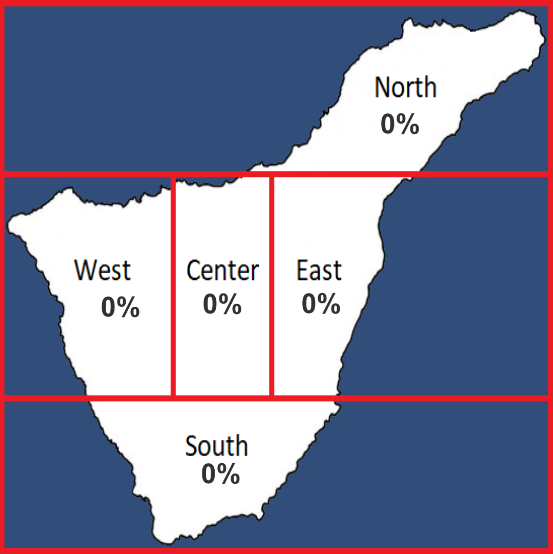
\includegraphics[width=0.25\textwidth]{Memoria_TFG_LaTeX/images/mapaNoCompleto.png}
    \caption{Demostración de cómo se verá el mapa cuando no se haya realizado ninguna visita.}
    \label{fig:mapaNoCompleto}
\end{figure}

Además, las zonas se irán rellenando, proporcionalmente a la cantidad de puntos de interés visitados dentro de esa zona, de un color azul.

\begin{figure}[H]
    \centering
    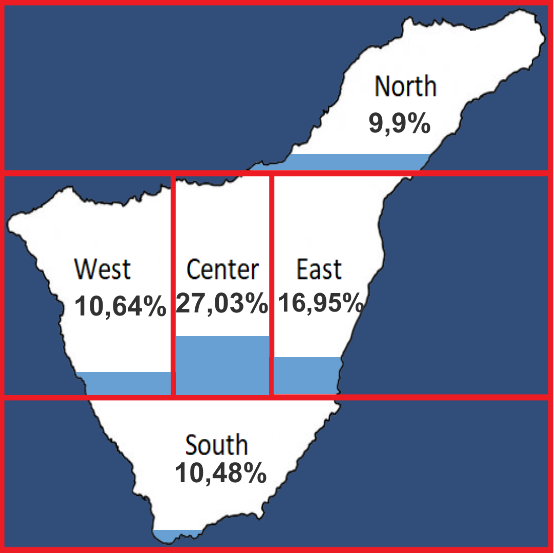
\includegraphics[width=0.25\textwidth]{Memoria_TFG_LaTeX/images/mapaParcial.png}
    \caption{Demostración de cómo se verá el mapa cuando se haya visitado cierta cantidad de puntos de cada zona.}
    \label{fig:mapaParcial}
\end{figure}

\begin{figure}[H]
    \centering
    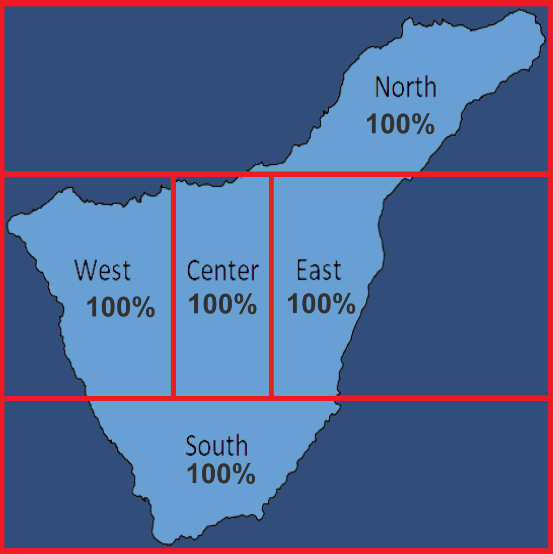
\includegraphics[width=0.25\textwidth]{Memoria_TFG_LaTeX/images/mapaCompleto.png}
    \caption{Demostración de cómo se verá el mapa una vez se hayan visitado todos los puntos de interés de la Isla al menos una vez}
    \label{fig:mapaCompleto}
\end{figure}

En la misma pantalla es posible observar diferentes estadísticas del usuario, como son:
\begin{itemize}
\item Número \textbf{total} de visitas realizadas, contabilizando varias visitas a un mismo punto.
\item Número de puntos de interés \textbf{diferentes} visitados.
\item La \textbf{zona} de la Isla más visitada.
\item El \textbf{tipo} de sitio de interés más visitado
\item El \textbf{sitio} de interés más visitado de todos.
\end{itemize}

\begin{figure}[H]
    \centering
    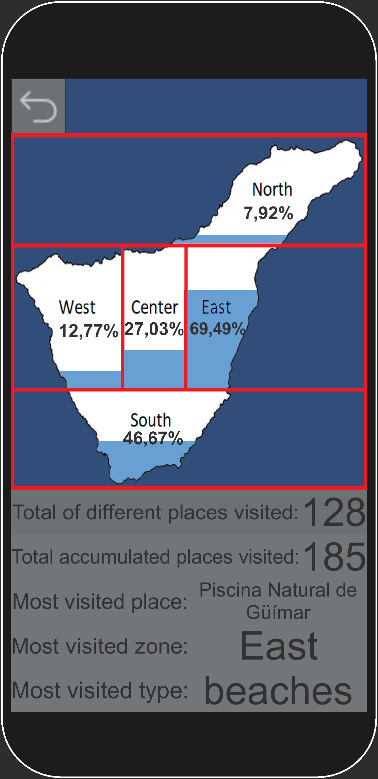
\includegraphics[width=0.25\textwidth]{Memoria_TFG_LaTeX/images/pantallaEstadisticas.png}
    \caption{Pantalla de las estadísticas ejecutándose en un emulador}
    \label{fig:pantallaEstadísticas}
\end{figure}

\newpage
\section{Recompensas}
\subsection{Rangos por nivel}
Los rangos de nivel dentro de la aplicación también presentan una forma de recompensar al usuario, haciéndole conocedor de su progreso gracias a la distinción de otros usuarios con menor rango.
Para establecer los rangos de nivel dentro de la aplicación se han utilizado los nombres de los diferentes niveles sociales que tenían los guanches\footnote{\textbf{Guanches}: Guanche es el nombre que se aplica a los antiguos aborígenes de la isla de Tenerife, Canarias, España, quienes la habitaban antes de la conquista castellana en 1496. Se trata de uno de los pueblos aborígenes de Canarias entroncados genética y culturalmente con los bereberes del norte de África.}.

La sociedad guanche era patriarcal\cite{sociedadguanche}, dividida en grupos sociales definidos por la riqueza, fundamentalmente la tierra y el ganado, en Tenerife existía una nobleza aborigen que está compuesta por:
\begin{itemize}
\item \textbf{Mencey} rey o monarca de cada uno de los territorios de la Isla o de la Isla entera.
\item \textbf{Achimencey} o gobernador, noble conformado en castas privilegiadas tanto en el ámbito político como religioso, participa en la toma de decisiones del gobierno.
\item \textbf{Guañameñes} o Guadameñas, sumos sacerdotes de los Menceyatos.
\item \textbf{Tagoreros} o Chaureros, corregidores y administradores de los diferentes Auchones.
\item \textbf{Sigoñes} o capitanes.
\item \textbf{Cichiciquitzos} o los guerreros, destinados al manejo de las armas.
\item \textbf{Achicaxna} o personal dedicado a la ganadería y la agricultura.
\item \textbf{Achicaxnais} dedicados a las tareas domésticas (Molineros, pescadores, alfareros, etc.). 
\item Embalsamadores, carniceros y mujeres eran las clases más bajas por su relación con la sangre.\cite{pou2017carniceros}
\end{itemize}

Siguiendo esta escala social he diseñado una serie de rangos diferenciados por puntuación:

\begin{ThreePartTable}
\label{table:rangos}
\captionof{table}{Puntos necesarios para alcanzar cada uno de los rangos}

\begin{tabularx}{0.9\textwidth} { 
  | >{\raggedright\arraybackslash}X
  | >{\raggedright\arraybackslash}X
  | >{\raggedright\arraybackslash}X
  | >{\raggedleft\arraybackslash}X | }
    \hline \textbf{Nombre Rango} & \textbf{Puntuación mínima}\\
    \hline Mencey                &  50.000\\
    \hline Achimencey            &  10.000\\
    \hline Guañameñe             &   3.000\\
    \hline Tagorero              &   1.500\\
    \hline Sigoñes               &     750\\
    \hline Cichiciquitzos        &     300\\
    \hline Achicaxna             &     100\\
    \hline Achicaxnais           &       0\\
    \hline 
\end{tabularx}
\end{ThreePartTable}
\begin{figure}[H]
    \centering
    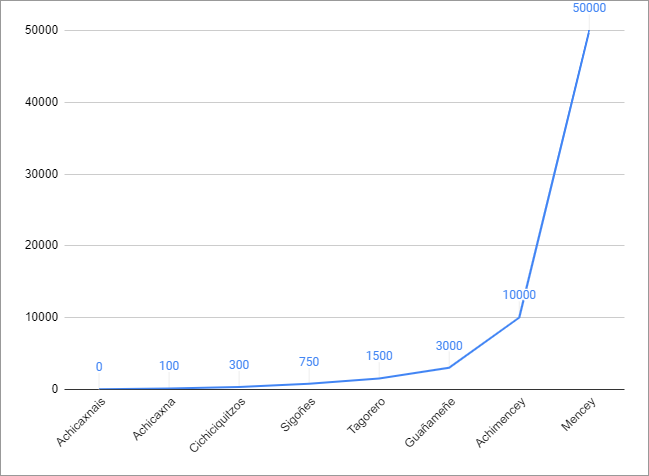
\includegraphics[width=1\textwidth]{Memoria_TFG_LaTeX/images/rangosGrafico.png}
    \caption{Diagrama que muestra el incremento de la puntuación requerida para pertenecer a un rango}
    \label{fig:puntosPorRango}
\end{figure}

Hay que destacar que, en el diseño de rangos, se ha buscado hacer que los rangos más bajos estén menos distanciados en cuanto a puntuación. Esto es así para hacer que los usuarios nuevos sientan que están progresando rápidamente cuando llevan poco tiempo usando la aplicación, de esta manera se consigue que los usuarios se familiaricen rápidamente con el sistema de rangos y, además, sientan cierta satisfacción por el rápido ascenso. Progresivamente, los siguientes rangos se van distanciando para hacer que, para los jugadores veteranos, siga siendo un reto moderadamente difícil e interesante subir de rango.
